
% Default to the notebook output style

    


% Inherit from the specified cell style.




    
\documentclass[11pt]{article}

    
    
    \usepackage[T1]{fontenc}
    % Nicer default font (+ math font) than Computer Modern for most use cases
    \usepackage{mathpazo}

    % Basic figure setup, for now with no caption control since it's done
    % automatically by Pandoc (which extracts ![](path) syntax from Markdown).
    \usepackage{graphicx}
    % We will generate all images so they have a width \maxwidth. This means
    % that they will get their normal width if they fit onto the page, but
    % are scaled down if they would overflow the margins.
    \makeatletter
    \def\maxwidth{\ifdim\Gin@nat@width>\linewidth\linewidth
    \else\Gin@nat@width\fi}
    \makeatother
    \let\Oldincludegraphics\includegraphics
    % Set max figure width to be 80% of text width, for now hardcoded.
    \renewcommand{\includegraphics}[1]{\Oldincludegraphics[width=.8\maxwidth]{#1}}
    % Ensure that by default, figures have no caption (until we provide a
    % proper Figure object with a Caption API and a way to capture that
    % in the conversion process - todo).
    \usepackage{caption}
    \DeclareCaptionLabelFormat{nolabel}{}
    \captionsetup{labelformat=nolabel}

    \usepackage{adjustbox} % Used to constrain images to a maximum size 
    \usepackage{xcolor} % Allow colors to be defined
    \usepackage{enumerate} % Needed for markdown enumerations to work
    \usepackage{geometry} % Used to adjust the document margins
    \usepackage{amsmath} % Equations
    \usepackage{amssymb} % Equations
    \usepackage{textcomp} % defines textquotesingle
    % Hack from http://tex.stackexchange.com/a/47451/13684:
    \AtBeginDocument{%
        \def\PYZsq{\textquotesingle}% Upright quotes in Pygmentized code
    }
    \usepackage{upquote} % Upright quotes for verbatim code
    \usepackage{eurosym} % defines \euro
    \usepackage[mathletters]{ucs} % Extended unicode (utf-8) support
    \usepackage[utf8x]{inputenc} % Allow utf-8 characters in the tex document
    \usepackage{fancyvrb} % verbatim replacement that allows latex
    \usepackage{grffile} % extends the file name processing of package graphics 
                         % to support a larger range 
    % The hyperref package gives us a pdf with properly built
    % internal navigation ('pdf bookmarks' for the table of contents,
    % internal cross-reference links, web links for URLs, etc.)
    \usepackage{hyperref}
    \usepackage{longtable} % longtable support required by pandoc >1.10
    \usepackage{booktabs}  % table support for pandoc > 1.12.2
    \usepackage[inline]{enumitem} % IRkernel/repr support (it uses the enumerate* environment)
    \usepackage[normalem]{ulem} % ulem is needed to support strikethroughs (\sout)
                                % normalem makes italics be italics, not underlines
    \usepackage{mathrsfs}
    

    
    
    % Colors for the hyperref package
    \definecolor{urlcolor}{rgb}{0,.145,.698}
    \definecolor{linkcolor}{rgb}{.71,0.21,0.01}
    \definecolor{citecolor}{rgb}{.12,.54,.11}

    % ANSI colors
    \definecolor{ansi-black}{HTML}{3E424D}
    \definecolor{ansi-black-intense}{HTML}{282C36}
    \definecolor{ansi-red}{HTML}{E75C58}
    \definecolor{ansi-red-intense}{HTML}{B22B31}
    \definecolor{ansi-green}{HTML}{00A250}
    \definecolor{ansi-green-intense}{HTML}{007427}
    \definecolor{ansi-yellow}{HTML}{DDB62B}
    \definecolor{ansi-yellow-intense}{HTML}{B27D12}
    \definecolor{ansi-blue}{HTML}{208FFB}
    \definecolor{ansi-blue-intense}{HTML}{0065CA}
    \definecolor{ansi-magenta}{HTML}{D160C4}
    \definecolor{ansi-magenta-intense}{HTML}{A03196}
    \definecolor{ansi-cyan}{HTML}{60C6C8}
    \definecolor{ansi-cyan-intense}{HTML}{258F8F}
    \definecolor{ansi-white}{HTML}{C5C1B4}
    \definecolor{ansi-white-intense}{HTML}{A1A6B2}
    \definecolor{ansi-default-inverse-fg}{HTML}{FFFFFF}
    \definecolor{ansi-default-inverse-bg}{HTML}{000000}

    % commands and environments needed by pandoc snippets
    % extracted from the output of `pandoc -s`
    \providecommand{\tightlist}{%
      \setlength{\itemsep}{0pt}\setlength{\parskip}{0pt}}
    \DefineVerbatimEnvironment{Highlighting}{Verbatim}{commandchars=\\\{\}}
    % Add ',fontsize=\small' for more characters per line
    \newenvironment{Shaded}{}{}
    \newcommand{\KeywordTok}[1]{\textcolor[rgb]{0.00,0.44,0.13}{\textbf{{#1}}}}
    \newcommand{\DataTypeTok}[1]{\textcolor[rgb]{0.56,0.13,0.00}{{#1}}}
    \newcommand{\DecValTok}[1]{\textcolor[rgb]{0.25,0.63,0.44}{{#1}}}
    \newcommand{\BaseNTok}[1]{\textcolor[rgb]{0.25,0.63,0.44}{{#1}}}
    \newcommand{\FloatTok}[1]{\textcolor[rgb]{0.25,0.63,0.44}{{#1}}}
    \newcommand{\CharTok}[1]{\textcolor[rgb]{0.25,0.44,0.63}{{#1}}}
    \newcommand{\StringTok}[1]{\textcolor[rgb]{0.25,0.44,0.63}{{#1}}}
    \newcommand{\CommentTok}[1]{\textcolor[rgb]{0.38,0.63,0.69}{\textit{{#1}}}}
    \newcommand{\OtherTok}[1]{\textcolor[rgb]{0.00,0.44,0.13}{{#1}}}
    \newcommand{\AlertTok}[1]{\textcolor[rgb]{1.00,0.00,0.00}{\textbf{{#1}}}}
    \newcommand{\FunctionTok}[1]{\textcolor[rgb]{0.02,0.16,0.49}{{#1}}}
    \newcommand{\RegionMarkerTok}[1]{{#1}}
    \newcommand{\ErrorTok}[1]{\textcolor[rgb]{1.00,0.00,0.00}{\textbf{{#1}}}}
    \newcommand{\NormalTok}[1]{{#1}}
    
    % Additional commands for more recent versions of Pandoc
    \newcommand{\ConstantTok}[1]{\textcolor[rgb]{0.53,0.00,0.00}{{#1}}}
    \newcommand{\SpecialCharTok}[1]{\textcolor[rgb]{0.25,0.44,0.63}{{#1}}}
    \newcommand{\VerbatimStringTok}[1]{\textcolor[rgb]{0.25,0.44,0.63}{{#1}}}
    \newcommand{\SpecialStringTok}[1]{\textcolor[rgb]{0.73,0.40,0.53}{{#1}}}
    \newcommand{\ImportTok}[1]{{#1}}
    \newcommand{\DocumentationTok}[1]{\textcolor[rgb]{0.73,0.13,0.13}{\textit{{#1}}}}
    \newcommand{\AnnotationTok}[1]{\textcolor[rgb]{0.38,0.63,0.69}{\textbf{\textit{{#1}}}}}
    \newcommand{\CommentVarTok}[1]{\textcolor[rgb]{0.38,0.63,0.69}{\textbf{\textit{{#1}}}}}
    \newcommand{\VariableTok}[1]{\textcolor[rgb]{0.10,0.09,0.49}{{#1}}}
    \newcommand{\ControlFlowTok}[1]{\textcolor[rgb]{0.00,0.44,0.13}{\textbf{{#1}}}}
    \newcommand{\OperatorTok}[1]{\textcolor[rgb]{0.40,0.40,0.40}{{#1}}}
    \newcommand{\BuiltInTok}[1]{{#1}}
    \newcommand{\ExtensionTok}[1]{{#1}}
    \newcommand{\PreprocessorTok}[1]{\textcolor[rgb]{0.74,0.48,0.00}{{#1}}}
    \newcommand{\AttributeTok}[1]{\textcolor[rgb]{0.49,0.56,0.16}{{#1}}}
    \newcommand{\InformationTok}[1]{\textcolor[rgb]{0.38,0.63,0.69}{\textbf{\textit{{#1}}}}}
    \newcommand{\WarningTok}[1]{\textcolor[rgb]{0.38,0.63,0.69}{\textbf{\textit{{#1}}}}}
    
    
    % Define a nice break command that doesn't care if a line doesn't already
    % exist.
    \def\br{\hspace*{\fill} \\* }
    % Math Jax compatibility definitions
    \def\gt{>}
    \def\lt{<}
    \let\Oldtex\TeX
    \let\Oldlatex\LaTeX
    \renewcommand{\TeX}{\textrm{\Oldtex}}
    \renewcommand{\LaTeX}{\textrm{\Oldlatex}}
    % Document parameters
    % Document title
    \title{Fractals \& Rendering Techniques}
    
    
    
    
    

    % Pygments definitions
    
\makeatletter
\def\PY@reset{\let\PY@it=\relax \let\PY@bf=\relax%
    \let\PY@ul=\relax \let\PY@tc=\relax%
    \let\PY@bc=\relax \let\PY@ff=\relax}
\def\PY@tok#1{\csname PY@tok@#1\endcsname}
\def\PY@toks#1+{\ifx\relax#1\empty\else%
    \PY@tok{#1}\expandafter\PY@toks\fi}
\def\PY@do#1{\PY@bc{\PY@tc{\PY@ul{%
    \PY@it{\PY@bf{\PY@ff{#1}}}}}}}
\def\PY#1#2{\PY@reset\PY@toks#1+\relax+\PY@do{#2}}

\expandafter\def\csname PY@tok@w\endcsname{\def\PY@tc##1{\textcolor[rgb]{0.73,0.73,0.73}{##1}}}
\expandafter\def\csname PY@tok@c\endcsname{\let\PY@it=\textit\def\PY@tc##1{\textcolor[rgb]{0.25,0.50,0.50}{##1}}}
\expandafter\def\csname PY@tok@cp\endcsname{\def\PY@tc##1{\textcolor[rgb]{0.74,0.48,0.00}{##1}}}
\expandafter\def\csname PY@tok@k\endcsname{\let\PY@bf=\textbf\def\PY@tc##1{\textcolor[rgb]{0.00,0.50,0.00}{##1}}}
\expandafter\def\csname PY@tok@kp\endcsname{\def\PY@tc##1{\textcolor[rgb]{0.00,0.50,0.00}{##1}}}
\expandafter\def\csname PY@tok@kt\endcsname{\def\PY@tc##1{\textcolor[rgb]{0.69,0.00,0.25}{##1}}}
\expandafter\def\csname PY@tok@o\endcsname{\def\PY@tc##1{\textcolor[rgb]{0.40,0.40,0.40}{##1}}}
\expandafter\def\csname PY@tok@ow\endcsname{\let\PY@bf=\textbf\def\PY@tc##1{\textcolor[rgb]{0.67,0.13,1.00}{##1}}}
\expandafter\def\csname PY@tok@nb\endcsname{\def\PY@tc##1{\textcolor[rgb]{0.00,0.50,0.00}{##1}}}
\expandafter\def\csname PY@tok@nf\endcsname{\def\PY@tc##1{\textcolor[rgb]{0.00,0.00,1.00}{##1}}}
\expandafter\def\csname PY@tok@nc\endcsname{\let\PY@bf=\textbf\def\PY@tc##1{\textcolor[rgb]{0.00,0.00,1.00}{##1}}}
\expandafter\def\csname PY@tok@nn\endcsname{\let\PY@bf=\textbf\def\PY@tc##1{\textcolor[rgb]{0.00,0.00,1.00}{##1}}}
\expandafter\def\csname PY@tok@ne\endcsname{\let\PY@bf=\textbf\def\PY@tc##1{\textcolor[rgb]{0.82,0.25,0.23}{##1}}}
\expandafter\def\csname PY@tok@nv\endcsname{\def\PY@tc##1{\textcolor[rgb]{0.10,0.09,0.49}{##1}}}
\expandafter\def\csname PY@tok@no\endcsname{\def\PY@tc##1{\textcolor[rgb]{0.53,0.00,0.00}{##1}}}
\expandafter\def\csname PY@tok@nl\endcsname{\def\PY@tc##1{\textcolor[rgb]{0.63,0.63,0.00}{##1}}}
\expandafter\def\csname PY@tok@ni\endcsname{\let\PY@bf=\textbf\def\PY@tc##1{\textcolor[rgb]{0.60,0.60,0.60}{##1}}}
\expandafter\def\csname PY@tok@na\endcsname{\def\PY@tc##1{\textcolor[rgb]{0.49,0.56,0.16}{##1}}}
\expandafter\def\csname PY@tok@nt\endcsname{\let\PY@bf=\textbf\def\PY@tc##1{\textcolor[rgb]{0.00,0.50,0.00}{##1}}}
\expandafter\def\csname PY@tok@nd\endcsname{\def\PY@tc##1{\textcolor[rgb]{0.67,0.13,1.00}{##1}}}
\expandafter\def\csname PY@tok@s\endcsname{\def\PY@tc##1{\textcolor[rgb]{0.73,0.13,0.13}{##1}}}
\expandafter\def\csname PY@tok@sd\endcsname{\let\PY@it=\textit\def\PY@tc##1{\textcolor[rgb]{0.73,0.13,0.13}{##1}}}
\expandafter\def\csname PY@tok@si\endcsname{\let\PY@bf=\textbf\def\PY@tc##1{\textcolor[rgb]{0.73,0.40,0.53}{##1}}}
\expandafter\def\csname PY@tok@se\endcsname{\let\PY@bf=\textbf\def\PY@tc##1{\textcolor[rgb]{0.73,0.40,0.13}{##1}}}
\expandafter\def\csname PY@tok@sr\endcsname{\def\PY@tc##1{\textcolor[rgb]{0.73,0.40,0.53}{##1}}}
\expandafter\def\csname PY@tok@ss\endcsname{\def\PY@tc##1{\textcolor[rgb]{0.10,0.09,0.49}{##1}}}
\expandafter\def\csname PY@tok@sx\endcsname{\def\PY@tc##1{\textcolor[rgb]{0.00,0.50,0.00}{##1}}}
\expandafter\def\csname PY@tok@m\endcsname{\def\PY@tc##1{\textcolor[rgb]{0.40,0.40,0.40}{##1}}}
\expandafter\def\csname PY@tok@gh\endcsname{\let\PY@bf=\textbf\def\PY@tc##1{\textcolor[rgb]{0.00,0.00,0.50}{##1}}}
\expandafter\def\csname PY@tok@gu\endcsname{\let\PY@bf=\textbf\def\PY@tc##1{\textcolor[rgb]{0.50,0.00,0.50}{##1}}}
\expandafter\def\csname PY@tok@gd\endcsname{\def\PY@tc##1{\textcolor[rgb]{0.63,0.00,0.00}{##1}}}
\expandafter\def\csname PY@tok@gi\endcsname{\def\PY@tc##1{\textcolor[rgb]{0.00,0.63,0.00}{##1}}}
\expandafter\def\csname PY@tok@gr\endcsname{\def\PY@tc##1{\textcolor[rgb]{1.00,0.00,0.00}{##1}}}
\expandafter\def\csname PY@tok@ge\endcsname{\let\PY@it=\textit}
\expandafter\def\csname PY@tok@gs\endcsname{\let\PY@bf=\textbf}
\expandafter\def\csname PY@tok@gp\endcsname{\let\PY@bf=\textbf\def\PY@tc##1{\textcolor[rgb]{0.00,0.00,0.50}{##1}}}
\expandafter\def\csname PY@tok@go\endcsname{\def\PY@tc##1{\textcolor[rgb]{0.53,0.53,0.53}{##1}}}
\expandafter\def\csname PY@tok@gt\endcsname{\def\PY@tc##1{\textcolor[rgb]{0.00,0.27,0.87}{##1}}}
\expandafter\def\csname PY@tok@err\endcsname{\def\PY@bc##1{\setlength{\fboxsep}{0pt}\fcolorbox[rgb]{1.00,0.00,0.00}{1,1,1}{\strut ##1}}}
\expandafter\def\csname PY@tok@kc\endcsname{\let\PY@bf=\textbf\def\PY@tc##1{\textcolor[rgb]{0.00,0.50,0.00}{##1}}}
\expandafter\def\csname PY@tok@kd\endcsname{\let\PY@bf=\textbf\def\PY@tc##1{\textcolor[rgb]{0.00,0.50,0.00}{##1}}}
\expandafter\def\csname PY@tok@kn\endcsname{\let\PY@bf=\textbf\def\PY@tc##1{\textcolor[rgb]{0.00,0.50,0.00}{##1}}}
\expandafter\def\csname PY@tok@kr\endcsname{\let\PY@bf=\textbf\def\PY@tc##1{\textcolor[rgb]{0.00,0.50,0.00}{##1}}}
\expandafter\def\csname PY@tok@bp\endcsname{\def\PY@tc##1{\textcolor[rgb]{0.00,0.50,0.00}{##1}}}
\expandafter\def\csname PY@tok@fm\endcsname{\def\PY@tc##1{\textcolor[rgb]{0.00,0.00,1.00}{##1}}}
\expandafter\def\csname PY@tok@vc\endcsname{\def\PY@tc##1{\textcolor[rgb]{0.10,0.09,0.49}{##1}}}
\expandafter\def\csname PY@tok@vg\endcsname{\def\PY@tc##1{\textcolor[rgb]{0.10,0.09,0.49}{##1}}}
\expandafter\def\csname PY@tok@vi\endcsname{\def\PY@tc##1{\textcolor[rgb]{0.10,0.09,0.49}{##1}}}
\expandafter\def\csname PY@tok@vm\endcsname{\def\PY@tc##1{\textcolor[rgb]{0.10,0.09,0.49}{##1}}}
\expandafter\def\csname PY@tok@sa\endcsname{\def\PY@tc##1{\textcolor[rgb]{0.73,0.13,0.13}{##1}}}
\expandafter\def\csname PY@tok@sb\endcsname{\def\PY@tc##1{\textcolor[rgb]{0.73,0.13,0.13}{##1}}}
\expandafter\def\csname PY@tok@sc\endcsname{\def\PY@tc##1{\textcolor[rgb]{0.73,0.13,0.13}{##1}}}
\expandafter\def\csname PY@tok@dl\endcsname{\def\PY@tc##1{\textcolor[rgb]{0.73,0.13,0.13}{##1}}}
\expandafter\def\csname PY@tok@s2\endcsname{\def\PY@tc##1{\textcolor[rgb]{0.73,0.13,0.13}{##1}}}
\expandafter\def\csname PY@tok@sh\endcsname{\def\PY@tc##1{\textcolor[rgb]{0.73,0.13,0.13}{##1}}}
\expandafter\def\csname PY@tok@s1\endcsname{\def\PY@tc##1{\textcolor[rgb]{0.73,0.13,0.13}{##1}}}
\expandafter\def\csname PY@tok@mb\endcsname{\def\PY@tc##1{\textcolor[rgb]{0.40,0.40,0.40}{##1}}}
\expandafter\def\csname PY@tok@mf\endcsname{\def\PY@tc##1{\textcolor[rgb]{0.40,0.40,0.40}{##1}}}
\expandafter\def\csname PY@tok@mh\endcsname{\def\PY@tc##1{\textcolor[rgb]{0.40,0.40,0.40}{##1}}}
\expandafter\def\csname PY@tok@mi\endcsname{\def\PY@tc##1{\textcolor[rgb]{0.40,0.40,0.40}{##1}}}
\expandafter\def\csname PY@tok@il\endcsname{\def\PY@tc##1{\textcolor[rgb]{0.40,0.40,0.40}{##1}}}
\expandafter\def\csname PY@tok@mo\endcsname{\def\PY@tc##1{\textcolor[rgb]{0.40,0.40,0.40}{##1}}}
\expandafter\def\csname PY@tok@ch\endcsname{\let\PY@it=\textit\def\PY@tc##1{\textcolor[rgb]{0.25,0.50,0.50}{##1}}}
\expandafter\def\csname PY@tok@cm\endcsname{\let\PY@it=\textit\def\PY@tc##1{\textcolor[rgb]{0.25,0.50,0.50}{##1}}}
\expandafter\def\csname PY@tok@cpf\endcsname{\let\PY@it=\textit\def\PY@tc##1{\textcolor[rgb]{0.25,0.50,0.50}{##1}}}
\expandafter\def\csname PY@tok@c1\endcsname{\let\PY@it=\textit\def\PY@tc##1{\textcolor[rgb]{0.25,0.50,0.50}{##1}}}
\expandafter\def\csname PY@tok@cs\endcsname{\let\PY@it=\textit\def\PY@tc##1{\textcolor[rgb]{0.25,0.50,0.50}{##1}}}

\def\PYZbs{\char`\\}
\def\PYZus{\char`\_}
\def\PYZob{\char`\{}
\def\PYZcb{\char`\}}
\def\PYZca{\char`\^}
\def\PYZam{\char`\&}
\def\PYZlt{\char`\<}
\def\PYZgt{\char`\>}
\def\PYZsh{\char`\#}
\def\PYZpc{\char`\%}
\def\PYZdl{\char`\$}
\def\PYZhy{\char`\-}
\def\PYZsq{\char`\'}
\def\PYZdq{\char`\"}
\def\PYZti{\char`\~}
% for compatibility with earlier versions
\def\PYZat{@}
\def\PYZlb{[}
\def\PYZrb{]}
\makeatother


    % Exact colors from NB
    \definecolor{incolor}{rgb}{0.0, 0.0, 0.5}
    \definecolor{outcolor}{rgb}{0.545, 0.0, 0.0}



    
    % Prevent overflowing lines due to hard-to-break entities
    \sloppy 
    % Setup hyperref package
    \hypersetup{
      breaklinks=true,  % so long urls are correctly broken across lines
      colorlinks=true,
      urlcolor=urlcolor,
      linkcolor=linkcolor,
      citecolor=citecolor,
      }
    % Slightly bigger margins than the latex defaults
    
    \geometry{verbose,tmargin=1in,bmargin=1in,lmargin=1in,rmargin=1in}
    
    

    \begin{document}
    	
    
    
    \maketitle
    \newpage
    \tableofcontents
    \newpage
    

    
    \hypertarget{introduction}{%
\section{Introduction}\label{introduction}}

    This document is an attempt at explaining different types of fractals
and techniques to create beautiful renderings.

First we start by explaining what shaders are and how you can program
them in GLSL. Then we will do a quick refresh on the math that is
required for complex numbers. If you think that math is not your thing,
the functions to do the complex arithmetic in GLSL are implemented in
this document and you can simply copy them. However, after the
Mandelbrot section there is no more escaping from the math, and basic
knowledge of algebra, vectors, and matrices will help tremendously.

Armed with the knowledge of basic GLSL programming and complex numbers,
we will start to render the Mandelbrot set. The core ideas of rendering
fractals are explained here. When we have a rendering of the set, we
will explore a technique for coloring. The coloring technique is
developed by \emph{Iniqo Quilez}, and I think it is so simple and
powerful that any programmer can benefit from it. To complete the
rendering program, we will also implement supersampling. With
supersampling we are `measuring' multiple points in the pixel and
average them out to get the final color. This gives an anti-aliasing
effect, where jagged edges become more smooth (less pixelized look).

    \hypertarget{shaders-and-glsl}{%
\section{Shaders and GLSL}\label{shaders-and-glsl}}

    https://thebookofshaders.com/01/

    \hypertarget{complex-numbers}{%
\section{Complex Numbers}\label{complex-numbers}}

    A complex number \(z\) is defined as a a number with two components,
indicating that they are two dimensional. An example is \(z=3+2i\),
which can be generalized to \(z=a + bi\). In a complex number, \(a\) is
called the \emph{real} component, and \(b\) is called the
\emph{imaginary} component. Like normal arithmetic, the rules for
addition and multiplication have been defined for complex numbers.
However, for complex numbers the arithmetic is differently from what you
are used to do with real numbers. How to do the arithmetic with complex
numbers is explained in a later section. Another notation that is used
in complex numbers is \(\textrm{Re}(z)\) to refer to the real component,
and \(\textrm{Im}(z)\) to refer to the imaginary component. This means
that a complex numbers can also be written as
\(z=\textrm{Re}(z) + i\ \textrm{Im}(z)\).

    \begin{quote}
Open a Python REPL, and define a complex number with
\texttt{complex(a,\ b)}. This is an easy way to play with complex
arithmetic.
\end{quote}

    \hypertarget{geometric-interpretation-of-complex-numbers}{%
\subsection{Geometric Interpretation of Complex
Numbers}\label{geometric-interpretation-of-complex-numbers}}

Another way to think about complex numbers, is with \(x\) and \(y\)
coordinates. In this idea the real component is the \(x\) value, and the
imaginary component is the \(y\) value. For example, \(z=3+2i\) can be
plotted on the complex plane:

    \begin{figure}[h]
\centering
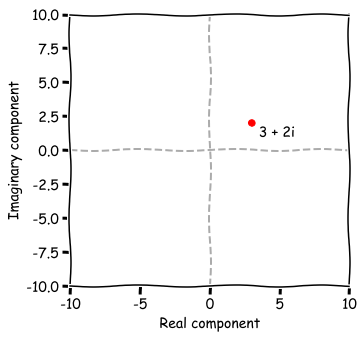
\includegraphics{img/complex-plane1.png}
\caption{\(3+2i\) in the complex plane}
\end{figure}

    This gives us a nice way to think about complex numbers. Namely, a
complex number can be thought of as a point in the \(xy\)-plane.

    \hypertarget{rules-of-complex-arithmetic}{%
\subsection{Rules of Complex
Arithmetic}\label{rules-of-complex-arithmetic}}

    Complex arithmetic is defined a bit differently from what you are used
to do with real numbers, because they are two dimensional. If have have
two complex numbers \(a + bi\) and \(c + di\), then:

\begin{itemize}
\tightlist
\item
  Addition: \((a + bi) + (c + di) = a + c + i(b + d)\).

  \begin{itemize}
  \tightlist
  \item
    Example: \((3 + 2i) + (1 - i) = 4 + i\).
  \end{itemize}
\item
  Multiplication:
  \((a + bi)(c + di) = ac + adi + bci + bdi^2 = ac - bd + i(ad + bc)\),
  notice that \(i^2 = -1\), thus \(bdi^2 = - bd\).

  \begin{itemize}
  \tightlist
  \item
    Example: \((3 + 2i)(1 - i) = 3 - 3i + 2i - 2i^2 = 5 - i\).
  \end{itemize}
\item
  Exponentiation:
  \((a + bi)^2 = a^2 + 2abi + b^2i^2 = a^2 - b^2 + 2abi\).

  \begin{itemize}
  \tightlist
  \item
    Example: \((3 + 2i)^2 = 9 + 6i + 6i + 4i^2 = 5 + 12i\).
  \end{itemize}
\end{itemize}

    \begin{quote}
Open a Python REPL and verify the examples to get a feel for it. It's
easier than you think.
\end{quote}

    \hypertarget{complex-arithmetic-in-glsl}{%
\subsection{Complex Arithmetic in
GLSL}\label{complex-arithmetic-in-glsl}}

    In GLSL we represent complex numbers with a vector of two components. If
we can encode the complex arithmetic in terms of matrix operations, the
calculations can be accelerated by the hardware of the GPU. In this
section, we will derive these matrix operations. For example, if we have
two complex numbers \(a + bi\) and \(c + di\), we can write this the
vectors \(u = [a, b]\) and \(v = [c, d]\).

\hypertarget{addition}{%
\subsubsection{Addition}\label{addition}}

The first case we will consider is addition. It can be achieved
trivially with vector addition. Both components will be added to each
other. Thus to add them the operation simply is \(u+v\).

\hypertarget{multiplication}{%
\subsubsection{Multiplication}\label{multiplication}}

The second case is multiplication. First we create a matrix
\(A = \begin{bmatrix} a && b \\ -b && a \end{bmatrix}\) from the vector
\(u\). For the complex multiplication of \(u\cdot v\), we replace \(u\)
with the matrix \(A\). When we work out the matrix multiplication:

\[ A\cdot v =  \begin{bmatrix} a && b \\ -b && a \end{bmatrix} \cdot \begin{bmatrix}c \\ d \end{bmatrix} = \begin{bmatrix} ac-bd \\ ad+bc \end{bmatrix},\]

the result is the same as the multiplication rule:
\((a + bi)(c + di) = ac - bd + i(ad + bc)\).

\hypertarget{exponentiation}{%
\subsubsection{Exponentiation}\label{exponentiation}}

The last case is exponentation. The case \(u\cdot u\) is a simplified
version of the multiplication case, since we can just multiply the
complex number by itself. Here we replace the first \(u\) with \(A\),
and work out \(A\cdot u\) to get:

\[ A\cdot u =  \begin{bmatrix} a && b \\ -b && a \end{bmatrix} \cdot \begin{bmatrix}a \\ b \end{bmatrix} = \begin{bmatrix} a^2-b^2 \\ 2ab \end{bmatrix},\]

which is the same as the exponentiation rule:
\((a + bi)^2 = a^2 - b^2 + 2abi\).

\hypertarget{implementation}{%
\subsubsection{Implementation}\label{implementation}}

The implementation in GLSL of the operations follows easily from the
formulas.

\begin{Shaded}
\begin{Highlighting}[]
\NormalTok{u + v                  }\CommentTok{// addition       u+v (vector addition)}
\DataTypeTok{mat2}\NormalTok{(u, -u.}\FunctionTok{y}\NormalTok{, u.}\FunctionTok{x}\NormalTok{) * v }\CommentTok{// multiplication u*v (matrix multiplication)}
\DataTypeTok{mat2}\NormalTok{(u, -u.}\FunctionTok{y}\NormalTok{, u.}\FunctionTok{x}\NormalTok{) * u }\CommentTok{// exponentiation u^2 (matrix multiplication)}
\end{Highlighting}
\end{Shaded}

    \hypertarget{the-mandelbrot-set}{%
\newpage
\section{The Mandelbrot Set}\label{the-mandelbrot-set}}

    Pick a complex number \(c\), for example \(c = 0.3 + 0.1i\), and
\(z = 0 + 0i\). For the first iteration we calculate \(z^2 + c\), which
is \((0 + 0i)^2 + 0.3 + 0.1i = 0.3 + 0.1i\). For the second iteration we
set \(z = 0.3+0.1i\), and then we find that \(z^2 + c = 0.38 + 0.16i\).
If we repeat this proces and plot the points we get after each
iteration:

\begin{figure}[h]
\centering
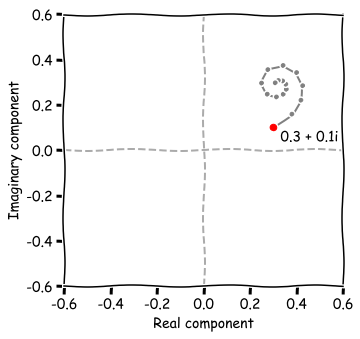
\includegraphics{img/orbit-converging.png}
\caption{Converging orbit}

\end{figure}

    As we can see the points are spiraling inwards to a point. The path that
the complex number takes when iterating is called the \emph{orbit}. It
is clear that the orbit is \emph{converging} towards a point. The other
case is that the orbit quickly grows after each iteration and soon
shoots off to infinity.

\begin{figure}[h]
\centering
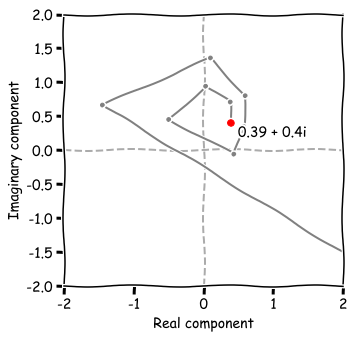
\includegraphics{img/orbit-diverging.png}
\caption{Diverging orbit}
\end{figure}

    If the point shoots to infinity, the point is not in the Mandelbrot set.
We can check this while iterating and it happens when \(|z| > B\). Based
on how fast the point shoots to infinity, and how many iterations we are
doing, a color is determined. We divide the iterations \(i\) by the
number of iterations \(N\), to get a value between \([0, 1]\). This
scalar value is used to map to a color. If the point stayed within the
bounds \(B\) during all iterations, it is in the Mandelbrot set and we
color it black.

    The proces we described above is perfectly suited for the GPU. Each
pixel on the screen, can be mapped, as an example to the range of
\([-2, 2]\) on the complex plane, and then we follow the orbit of that
complex number when we iterate with the Mandelbrot formula.

    The Mandelbrot set is given with:

\[ z_{n+1} = z_n^2 + c \]

Clasically we pick a bound \(B=2\) which is the disk that contains the
Mandelbrot set. To remove this disc, we increase \(B\) to \(4\). On each
iteration we calculate \(z = z^2 + c\), and check if \(|z|\) is greater
than \(B\), meaning that the orbit of \(z\) has escaped to infinity.
This happens when \(\sqrt{a^2 + b^2} > B\), which we can square to get
\(a^2 + b^2 > B^2\). The next thing we can do is to rewrite
\(a^2 + b^2\) as the dot product \(z\cdot z\). This leads to the
following equation that we can use to check if \(z\) has escaped to
infinity: \(z\cdot z > B^2\). Rewriting it algebraically removes the
necessity of the square root operation, which improves the speed of the
algorithm.

    The following GLSL code is a simple and fast implementation for
rendering the Mandelbrot set.

    \begin{Shaded}
\begin{Highlighting}[]
\PreprocessorTok{#define N 64.}
\PreprocessorTok{#define B 4.}

\DataTypeTok{void} \FunctionTok{mainImage}\NormalTok{( }\DataTypeTok{out} \DataTypeTok{vec4}\NormalTok{ fragColor, }\DataTypeTok{in} \DataTypeTok{vec2}\NormalTok{ fragCoord ) \{}
    
    \DataTypeTok{vec2}\NormalTok{ R = iResolution.}\FunctionTok{xy}\NormalTok{;}
    \DataTypeTok{vec2}\NormalTok{ uv = (}\FloatTok{2.}\NormalTok{ * fragCoord - R - }\FloatTok{1.}\NormalTok{) / R.}\FunctionTok{y}\NormalTok{;}
    \DataTypeTok{vec2}\NormalTok{ z = }\DataTypeTok{vec2}\NormalTok{(}\DecValTok{0}\NormalTok{), c = uv;}
    \DataTypeTok{float}\NormalTok{ i;}

    \KeywordTok{for}\NormalTok{(i=}\FloatTok{0.}\NormalTok{; i < N; i++) \{}
\NormalTok{        z = }\DataTypeTok{mat2}\NormalTok{(z, -z.}\FunctionTok{y}\NormalTok{, z.}\FunctionTok{x}\NormalTok{) * z + c;}
        \KeywordTok{if}\NormalTok{(}\BuiltInTok{dot}\NormalTok{(z, z) > B*B) }\KeywordTok{break}\NormalTok{;}
\NormalTok{    \}}
    
    \KeywordTok{if}\NormalTok{(i==N) \{ i = }\FloatTok{0.}\NormalTok{; \} }\CommentTok{// mark interior black}
\NormalTok{    fragColor = }\DataTypeTok{vec4}\NormalTok{(}\DataTypeTok{vec3}\NormalTok{(i/N), }\FloatTok{1.}\NormalTok{);}
\NormalTok{\}}
\end{Highlighting}
\end{Shaded}

    It will render the following image:

    \begin{figure}[h]
\centering
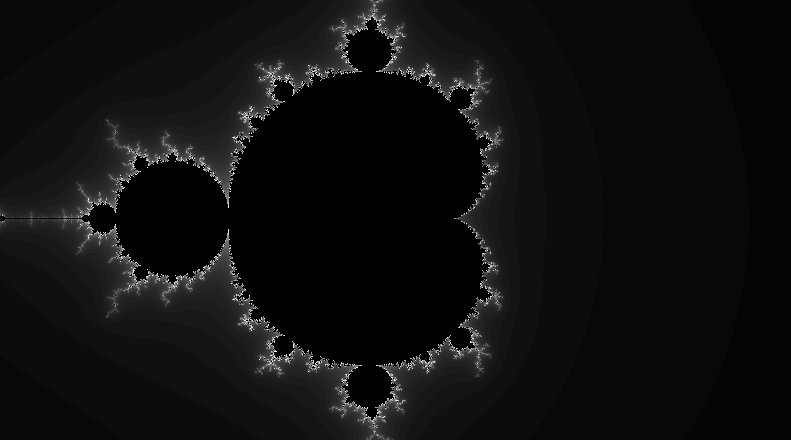
\includegraphics{img/mandelbrot-first.png}
\caption{Simple Mandelbrot}
\end{figure}

    The code can be refactored a little bit by moving iteration into a new
function \texttt{iterate(float\ p)}. We can also scale the image by
multiplying \texttt{uv} by \(1.2\). Finally, to center the image we
subtract \([0.4, 0.0]\) from \texttt{uv}. This results in the final code
for this section:

    \begin{Shaded}
\begin{Highlighting}[]
\PreprocessorTok{#define N 64.}
\PreprocessorTok{#define B 4.}

\DataTypeTok{float} \FunctionTok{iterate}\NormalTok{(}\DataTypeTok{vec2}\NormalTok{ p) \{}
    \DataTypeTok{vec2}\NormalTok{ z = }\DataTypeTok{vec2}\NormalTok{(}\DecValTok{0}\NormalTok{), c = p;}
    \DataTypeTok{float}\NormalTok{ i;}
    \KeywordTok{for}\NormalTok{(i=}\FloatTok{0.}\NormalTok{; i < N; i++) \{}
\NormalTok{        z = }\DataTypeTok{mat2}\NormalTok{(z, -z.}\FunctionTok{y}\NormalTok{, z.}\FunctionTok{x}\NormalTok{) * z + c;}
        \KeywordTok{if}\NormalTok{(}\BuiltInTok{dot}\NormalTok{(z, z) > B*B) }\KeywordTok{break}\NormalTok{;}
\NormalTok{    \}}
    \KeywordTok{return}\NormalTok{ i;       }
\NormalTok{\}}

\DataTypeTok{void} \FunctionTok{mainImage}\NormalTok{( }\DataTypeTok{out} \DataTypeTok{vec4}\NormalTok{ fragColor, }\DataTypeTok{in} \DataTypeTok{vec2}\NormalTok{ fragCoord ) \{}
    
    \DataTypeTok{vec2}\NormalTok{ R = iResolution.}\FunctionTok{xy}\NormalTok{;}
    \DataTypeTok{vec2}\NormalTok{ uv = }\FloatTok{1.2}\NormalTok{ * (}\FloatTok{2.}\NormalTok{ * fragCoord - R - }\FloatTok{1.}\NormalTok{) / R.}\FunctionTok{y}\NormalTok{ - }\DataTypeTok{vec2}\NormalTok{(.}\FunctionTok{4}\NormalTok{, }\FloatTok{0.}\NormalTok{);}

    \DataTypeTok{float}\NormalTok{ n = }\FunctionTok{iterate}\NormalTok{(uv) / N;}
    \KeywordTok{if}\NormalTok{(n==}\FloatTok{1.}\NormalTok{) n = }\FloatTok{0.}\NormalTok{;}
\NormalTok{    fragColor = }\DataTypeTok{vec4}\NormalTok{(}\DataTypeTok{vec3}\NormalTok{(n), }\FloatTok{1.0}\NormalTok{);}
\NormalTok{\}}
\end{Highlighting}
\end{Shaded}

    The end result should look like this:

    \begin{figure}[h]
\centering
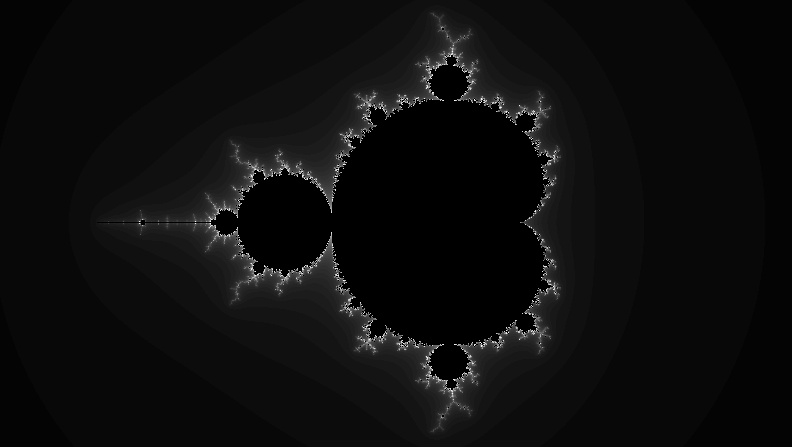
\includegraphics{img/mandelbrot-centered.png}
\caption{Centered Mandelbrot}
\end{figure}

    So far we have created the Mandelbrot itself, but the white coloring is
quite boring. In the next section we will explore a technique which
allows us to create color gradients with a surprisingly simple formula.

    \hypertarget{colorful-palettes}{%
\section{Colorful Palettes}\label{colorful-palettes}}

    When we calculated the Mandelbrot set, we apply colorization based on
the value of \(n\), which has been normalized between \([0,1]\). The
idea in this chapter is to develop a function with a parameter \(t\)
ranging between \([0,1]\), that returns a color from a gradient. The
gradient can be composed out of many different colors, also called a
\emph{palette}.

    \hypertarget{procedural-color-palette}{%
\subsection{Procedural Color Palette}\label{procedural-color-palette}}

    A simple way to create a procedural color palette has been created by
\emph{Inoqo Quilez}
(https://iquilezles.org/www/articles/palettes/palettes.htm), it is the
following cosine expression:

    \[ \textrm{color}(t) = a + b \cdot \cos [2\pi(c\cdot t+d)] \]

    As \(t\) runs from \(0\) to \(1\), the cosine oscillates \(c\) times
with a phase of \(d\). The result is scaled and biased by \(a\) and
\(b\) to meet the desired contrast and brightness. The parameters
\(a, b, c\) and \(d\) are vectors with three components (r, g, b). We
can also think of \(a\) as the \emph{offset}, \(b\) as the
\emph{amplitude}, \(c\) as the \emph{frequency}, and \(d\) as the
\emph{phase}, for each r, g, b component respectively.

    For example, if we pick values for \(a, b, c\) and \(d\):

    \[ a = \begin{bmatrix} 0.65 \\ 0.5 \\ 0.31 \end{bmatrix} \quad b = \begin{bmatrix} -0.65 \\ 0.5 \\ 0.6 \end{bmatrix} \quad c = \begin{bmatrix} 0.333 \\ 0.278 \\ 0.278 \end{bmatrix} \quad d = \begin{bmatrix} 0.66 \\ 0 \\ 0.667 \end{bmatrix} \]

    we can create a plot with the
\href{http://dev.thi.ng/gradients/}{\emph{cosine gradient generator}}.
This gives a nice visualization of what is going on and how this
procedural color palette works.

    \begin{figure}[h]
\centering
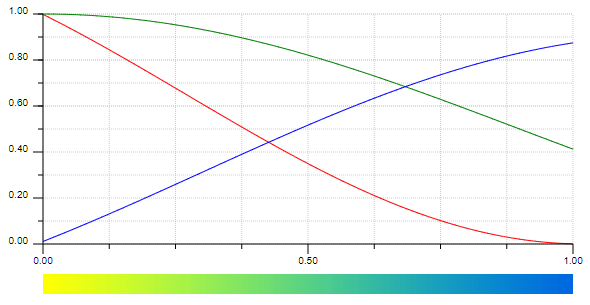
\includegraphics{img/color-palette.png}
\caption{Color palette}
\end{figure}

    We can see that each of the r, g, b components sits on a cosine wave and
they are mixed together with sliding \(t\) between \([0,1]\). This set
of values gives a nice yellow, green and blueish gradient.

    \hypertarget{gradient-examples}{%
\subsection{Gradient Examples}\label{gradient-examples}}

    This section contains a table with different palettes that can be used
as a color map.

    \begin{longtable}[]{@{}lllll@{}}
\toprule
\begin{minipage}[b]{0.17\columnwidth}\raggedright
a\strut
\end{minipage} & \begin{minipage}[b]{0.17\columnwidth}\raggedright
b\strut
\end{minipage} & \begin{minipage}[b]{0.17\columnwidth}\raggedright
c\strut
\end{minipage} & \begin{minipage}[b]{0.17\columnwidth}\raggedright
d\strut
\end{minipage} & \begin{minipage}[b]{0.17\columnwidth}\raggedright
palette\strut
\end{minipage}\tabularnewline
\midrule
\endhead
\begin{minipage}[t]{0.17\columnwidth}\raggedright
\texttt{{[}0.\ \ 0.5\ 0.5{]}}\strut
\end{minipage} & \begin{minipage}[t]{0.17\columnwidth}\raggedright
\texttt{{[}0.\ \ 0.5\ 0.5{]}}\strut
\end{minipage} & \begin{minipage}[t]{0.17\columnwidth}\raggedright
\texttt{{[}0.\ \ \ 0.5\ \ 0.33{]}}\strut
\end{minipage} & \begin{minipage}[t]{0.17\columnwidth}\raggedright
\texttt{{[}0.\ \ \ 0.5\ \ 0.66{]}}\strut
\end{minipage} & \begin{minipage}[t]{0.17\columnwidth}\raggedright

\includegraphics{palettes/palette1.png}\strut
\end{minipage}\tabularnewline
\begin{minipage}[t]{0.17\columnwidth}\raggedright
\texttt{{[}0.938\ 0.328\ 0.718{]}}\strut
\end{minipage} & \begin{minipage}[t]{0.17\columnwidth}\raggedright
\texttt{{[}0.659\ 0.438\ 0.328{]}}\strut
\end{minipage} & \begin{minipage}[t]{0.17\columnwidth}\raggedright
\texttt{{[}0.388\ 0.388\ 0.296{]}}\strut
\end{minipage} & \begin{minipage}[t]{0.17\columnwidth}\raggedright
\texttt{{[}2.538\ 2.478\ 0.168{]}}\strut
\end{minipage} & \begin{minipage}[t]{0.17\columnwidth}\raggedright

\includegraphics{palettes/palette2.png}\strut
\end{minipage}\tabularnewline
\begin{minipage}[t]{0.17\columnwidth}\raggedright
\texttt{{[}0.66\ 0.56\ 0.68{]}}\strut
\end{minipage} & \begin{minipage}[t]{0.17\columnwidth}\raggedright
\texttt{{[}0.718\ 0.438\ 0.72\ {]}}\strut
\end{minipage} & \begin{minipage}[t]{0.17\columnwidth}\raggedright
\texttt{{[}0.52\ 0.8\ \ 0.52{]}}\strut
\end{minipage} & \begin{minipage}[t]{0.17\columnwidth}\raggedright
\texttt{{[}-0.43\ \ -0.397\ -0.083{]}}\strut
\end{minipage} & \begin{minipage}[t]{0.17\columnwidth}\raggedright

\includegraphics{palettes/palette3.png}\strut
\end{minipage}\tabularnewline
\begin{minipage}[t]{0.17\columnwidth}\raggedright
\texttt{{[}0.5\ 0.5\ 0.5{]}}\strut
\end{minipage} & \begin{minipage}[t]{0.17\columnwidth}\raggedright
\texttt{{[}0.5\ 0.5\ 0.5{]}}\strut
\end{minipage} & \begin{minipage}[t]{0.17\columnwidth}\raggedright
\texttt{{[}0.8\ 0.8\ 0.5{]}}\strut
\end{minipage} & \begin{minipage}[t]{0.17\columnwidth}\raggedright
\texttt{{[}0.\ \ 0.2\ 0.5{]}}\strut
\end{minipage} & \begin{minipage}[t]{0.17\columnwidth}\raggedright

\includegraphics{palettes/palette4.png}\strut
\end{minipage}\tabularnewline
\begin{minipage}[t]{0.17\columnwidth}\raggedright
\texttt{{[}0.821\ 0.328\ 0.242{]}}\strut
\end{minipage} & \begin{minipage}[t]{0.17\columnwidth}\raggedright
\texttt{{[}0.659\ 0.481\ 0.896{]}}\strut
\end{minipage} & \begin{minipage}[t]{0.17\columnwidth}\raggedright
\texttt{{[}0.612\ 0.34\ \ 0.296{]}}\strut
\end{minipage} & \begin{minipage}[t]{0.17\columnwidth}\raggedright
\texttt{{[}\ 2.82\ \ \ 3.026\ -0.273{]}}\strut
\end{minipage} & \begin{minipage}[t]{0.17\columnwidth}\raggedright

\includegraphics{palettes/palette5.png}\strut
\end{minipage}\tabularnewline
\begin{minipage}[t]{0.17\columnwidth}\raggedright
\texttt{{[}0.5\ 0.5\ 0.5{]}}\strut
\end{minipage} & \begin{minipage}[t]{0.17\columnwidth}\raggedright
\texttt{{[}0.5\ 0.5\ 0.5{]}}\strut
\end{minipage} & \begin{minipage}[t]{0.17\columnwidth}\raggedright
\texttt{{[}1.\ 1.\ 1.{]}}\strut
\end{minipage} & \begin{minipage}[t]{0.17\columnwidth}\raggedright
\texttt{{[}0.\ \ \ 0.33\ 0.67{]}}\strut
\end{minipage} & \begin{minipage}[t]{0.17\columnwidth}\raggedright

\includegraphics{palettes/palette6.png}\strut
\end{minipage}\tabularnewline
\begin{minipage}[t]{0.17\columnwidth}\raggedright
\texttt{{[}0.5\ 0.5\ 0.5{]}}\strut
\end{minipage} & \begin{minipage}[t]{0.17\columnwidth}\raggedright
\texttt{{[}0.5\ 0.5\ 0.5{]}}\strut
\end{minipage} & \begin{minipage}[t]{0.17\columnwidth}\raggedright
\texttt{{[}1.\ 1.\ 1.{]}}\strut
\end{minipage} & \begin{minipage}[t]{0.17\columnwidth}\raggedright
\texttt{{[}0.\ \ 0.1\ 0.2{]}}\strut
\end{minipage} & \begin{minipage}[t]{0.17\columnwidth}\raggedright

\includegraphics{palettes/palette7.png}\strut
\end{minipage}\tabularnewline
\begin{minipage}[t]{0.17\columnwidth}\raggedright
\texttt{{[}0.5\ 0.5\ 0.5{]}}\strut
\end{minipage} & \begin{minipage}[t]{0.17\columnwidth}\raggedright
\texttt{{[}0.5\ 0.5\ 0.5{]}}\strut
\end{minipage} & \begin{minipage}[t]{0.17\columnwidth}\raggedright
\texttt{{[}1.\ 1.\ 1.{]}}\strut
\end{minipage} & \begin{minipage}[t]{0.17\columnwidth}\raggedright
\texttt{{[}0.3\ 0.2\ 0.2{]}}\strut
\end{minipage} & \begin{minipage}[t]{0.17\columnwidth}\raggedright

\includegraphics{palettes/palette8.png}\strut
\end{minipage}\tabularnewline
\begin{minipage}[t]{0.17\columnwidth}\raggedright
\texttt{{[}0.5\ 0.5\ 0.5{]}}\strut
\end{minipage} & \begin{minipage}[t]{0.17\columnwidth}\raggedright
\texttt{{[}0.5\ 0.5\ 0.5{]}}\strut
\end{minipage} & \begin{minipage}[t]{0.17\columnwidth}\raggedright
\texttt{{[}1.\ 1.\ 1.{]}}\strut
\end{minipage} & \begin{minipage}[t]{0.17\columnwidth}\raggedright
\texttt{{[}0.8\ 0.9\ 0.3{]}}\strut
\end{minipage} & \begin{minipage}[t]{0.17\columnwidth}\raggedright
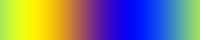
\includegraphics{palettes/palette9.png}\strut
\end{minipage}\tabularnewline
\begin{minipage}[t]{0.17\columnwidth}\raggedright
\texttt{{[}0.5\ 0.5\ 0.5{]}}\strut
\end{minipage} & \begin{minipage}[t]{0.17\columnwidth}\raggedright
\texttt{{[}0.5\ 0.5\ 0.5{]}}\strut
\end{minipage} & \begin{minipage}[t]{0.17\columnwidth}\raggedright
\texttt{{[}1.\ \ 0.7\ 0.4{]}}\strut
\end{minipage} & \begin{minipage}[t]{0.17\columnwidth}\raggedright
\texttt{{[}0.\ \ \ 0.15\ 0.2\ {]}}\strut
\end{minipage} & \begin{minipage}[t]{0.17\columnwidth}\raggedright

\includegraphics{palettes/palette10.png}\strut
\end{minipage}\tabularnewline
\begin{minipage}[t]{0.17\columnwidth}\raggedright
\texttt{{[}0.5\ 0.5\ 0.5{]}}\strut
\end{minipage} & \begin{minipage}[t]{0.17\columnwidth}\raggedright
\texttt{{[}0.5\ 0.5\ 0.5{]}}\strut
\end{minipage} & \begin{minipage}[t]{0.17\columnwidth}\raggedright
\texttt{{[}2.\ 1.\ 0.{]}}\strut
\end{minipage} & \begin{minipage}[t]{0.17\columnwidth}\raggedright
\texttt{{[}0.5\ \ 0.2\ \ 0.25{]}}\strut
\end{minipage} & \begin{minipage}[t]{0.17\columnwidth}\raggedright

\includegraphics{palettes/palette11.png}\strut
\end{minipage}\tabularnewline
\begin{minipage}[t]{0.17\columnwidth}\raggedright
\texttt{{[}0.5\ 0.5\ 0.5{]}}\strut
\end{minipage} & \begin{minipage}[t]{0.17\columnwidth}\raggedright
\texttt{{[}0.5\ 0.5\ 0.5{]}}\strut
\end{minipage} & \begin{minipage}[t]{0.17\columnwidth}\raggedright
\texttt{{[}2.\ 1.\ 1.{]}}\strut
\end{minipage} & \begin{minipage}[t]{0.17\columnwidth}\raggedright
\texttt{{[}0.\ \ \ 0.25\ 0.25{]}}\strut
\end{minipage} & \begin{minipage}[t]{0.17\columnwidth}\raggedright

\includegraphics{palettes/palette12.png}\strut
\end{minipage}\tabularnewline
\bottomrule
\end{longtable}

    This is a list of palettes have been created by
http://dev.thi.ng/gradients, and \emph{Iniqo Quilez}. More gradients can
be created with http://dev.thi.ng/gradients.

    \hypertarget{implementation}{%
\subsection{Implementation}\label{implementation}}

    The code follows easily from the formula described above:

    \begin{Shaded}
\begin{Highlighting}[]
\DataTypeTok{vec3} \FunctionTok{palette}\NormalTok{( }\DataTypeTok{in} \DataTypeTok{float}\NormalTok{ t, }\DataTypeTok{in} \DataTypeTok{vec3}\NormalTok{ a, }\DataTypeTok{in} \DataTypeTok{vec3}\NormalTok{ b, }\DataTypeTok{in} \DataTypeTok{vec3}\NormalTok{ c, }\DataTypeTok{in} \DataTypeTok{vec3}\NormalTok{ d )}
\NormalTok{\{}
    \KeywordTok{return}\NormalTok{ a + b*}\BuiltInTok{cos}\NormalTok{( }\FloatTok{6.28318}\NormalTok{*(c*t+d) );}
\NormalTok{\}}
\end{Highlighting}
\end{Shaded}

    \hypertarget{smooth-iteration-count}{%
\section{Smooth Iteration Count}\label{smooth-iteration-count}}

    As you probably have noticed, the change in color goes in discrete
steps, which creates the color bands. This happens because \(n\), the
number of iterations, is an integer. These discrete steps of changes in
colors results in the rendering of the bands. To solve this problem,
\href{https://iquilezles.org/www/articles/mset_smooth/mset_smooth.htm}{\emph{Iniqo
Quilez} explains a method} that determines the fractional part of \(n\).
We subtract the fractional part from \(n\) to get \(sn\), which is
smooth.

    The fractional part of the smooth iteration count can be calculated
with:

    \[ sn = n - \dfrac{\ln \dfrac{\ln |z_n|}{\ln B}}{\ln d} \]

    where \(B\) is the threshold when \(|z|\) has escaped, and \(d\) is the
degree of the polynomial under iteration. In the case where \(d=2\),
such as in the Mandelbrot set, an optimized variant is available:

    \[ sn = n - \log_2\log_2(z_n^2)+k \]

Implementing the non-optimized version can be done by having the line in
the \texttt{iterate} function:

\begin{Shaded}
\begin{Highlighting}[]
\KeywordTok{return}\NormalTok{ i;}
\end{Highlighting}
\end{Shaded}

perform the formula we described above, which in GLSL is:

\begin{Shaded}
\begin{Highlighting}[]
\KeywordTok{return}\NormalTok{ i - }\BuiltInTok{log}\NormalTok{(}\BuiltInTok{log}\NormalTok{(}\BuiltInTok{dot}\NormalTok{(z, z)) / }\BuiltInTok{log}\NormalTok{(B)) / }\BuiltInTok{log}\NormalTok{(}\FloatTok{2.}\NormalTok{);  }
\end{Highlighting}
\end{Shaded}

    The next image is a rendering of a comparison between both methods. The
smooth iteration count can be seen in the top part of the rendering, and
the integer iteration count in the bottom half.

    \begin{figure}[h]
\centering

\includegraphics{img/smooth-iteration-count.png}
\caption{Mandelbrot Smooth Iteration Count}
\end{figure}

    \hypertarget{supersampling}{%
\section{Supersampling}\label{supersampling}}

    \hypertarget{burning-ship-fractal}{%
\section{Burning Ship Fractal}\label{burning-ship-fractal}}

    \hypertarget{julia-sets}{%
\section{Julia Sets}\label{julia-sets}}

    \hypertarget{animation}{%
\section{Animation}\label{animation}}

    \hypertarget{rotation-over-time}{%
\subsection{Rotation over time}\label{rotation-over-time}}

    \hypertarget{zoom-over-time}{%
\subsection{Zoom over time}\label{zoom-over-time}}

    \hypertarget{polynomials}{%
\section{Polynomials}\label{polynomials}}

    \begin{figure}[h]
\centering
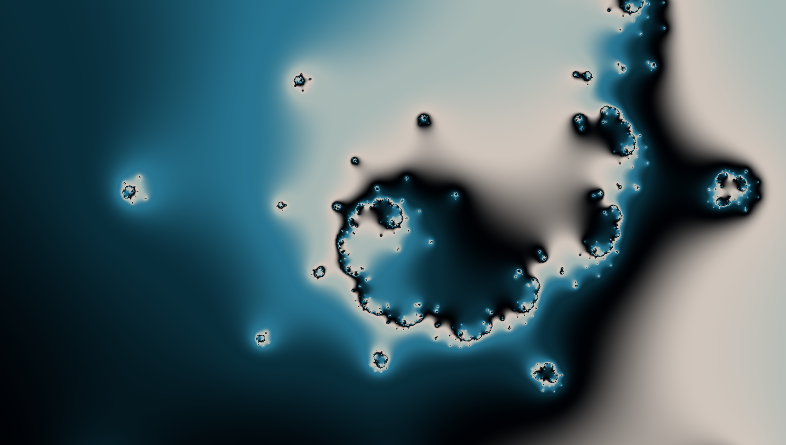
\includegraphics{img/poly1.png}
\caption{Polynomial - Spiral}
\end{figure}

    \hypertarget{distance-rendering}{%
\section{Distance Rendering}\label{distance-rendering}}

    https://iquilezles.org/www/articles/distancefractals/distancefractals.htm

    \hypertarget{geometric-orbit-traps}{%
\section{Geometric Orbit Traps}\label{geometric-orbit-traps}}

    https://iquilezles.org/www/articles/ftrapsgeometric/ftrapsgeometric.htm

    \hypertarget{iterated-functions-systems}{%
\section{Iterated Functions Systems}\label{iterated-functions-systems}}

    https://iquilezles.org/www/articles/ifsfractals/ifsfractals.htm

    \hypertarget{references}{%
\section{References}\label{references}}


    % Add a bibliography block to the postdoc
    
    
    
    \end{document}
